\documentclass[10pt]{article}\usepackage[margin=.7in]{geometry}\usepackage{graphicx}\begin{document}\section*{Weighted degree-one doubling}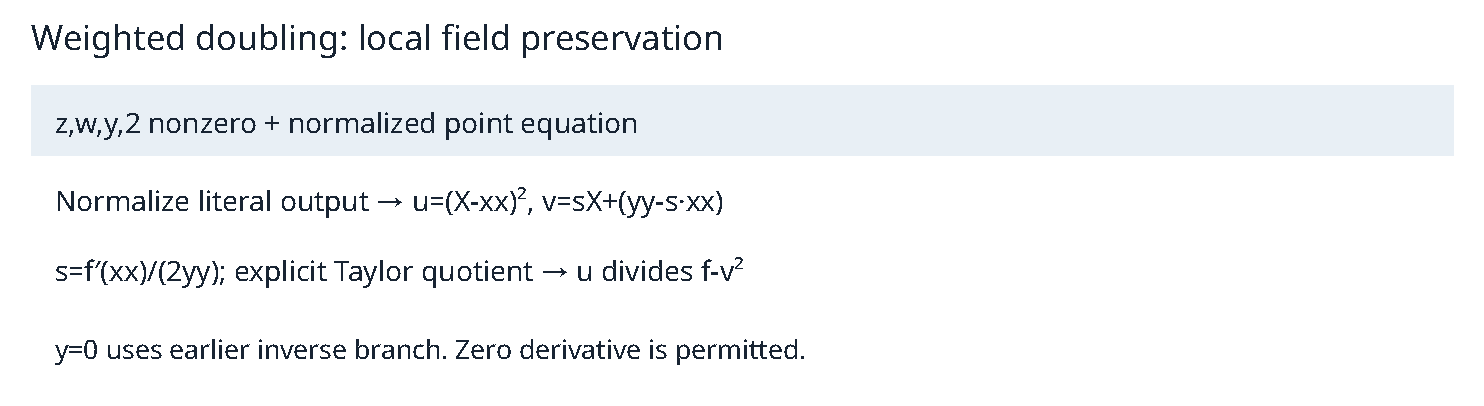
\includegraphics[width=\linewidth]{figure.pdf}
Seven Lean declarations compile. Separate controls and axiom readback return exit zero. The weighted field formula preserves normalized Mumford divisibility on $f=X^5+a_3X^3+a_2X^2+a_1X+a_0$ under the displayed assumptions.

\paragraph{Construction} The output has $z'=z$, $w'=2y$. Its normalized quadratic is $(X-xx)^2$ and its linear polynomial is the tangent interpolant. An explicit quotient identity proves divisibility; input point validity and the tangent equation cancel the residual terms.

\paragraph{Branches and controls} Self-add with nonzero ordinate reaches doubling; zero ordinate reaches the earlier inverse branch. A nonunit-weight fixture instantiates the full theorem. A separate zero-derivative fixture also instantiates it. Derivative nonvanishing is not a required denominator condition.

\paragraph{Scope} This is field polynomial validity. Global nonsingularity and class-sum interpretation are separate; UInt64 execution, counters, compiler and walk closure are not proved. The curve preprocessing is not included. The guard lemma covers self-add, not every differently weighted equal-point input. The first algebra fixture uses $f=X^5$ and is not presented as a smooth curve.

\paragraph{Evidence} Initial failed attempt retained; corrected modules, controls and readback pass. Only standard Lean axioms occur. REPORT.md records exact formula/source boundaries and literature equation(3); sources.json and the manifest bind artifacts. Independent review pending. No scientific trials or repository edits.
\end{document}